\subsection{Problem discussion, in the Sokoban domain}
Sokoban is a game originating from Japan. The essence of the game is to push jewels around in a room containing obstacles, in a manner that will enable the player to place all the jewels on so called goals in the room. See figure \ref{fig:sokohero} for a screenshot of a sokoban game.
Sokoban is an interesting game to study in the domain of Artificial Intelligence, because it presents a so called NP-complete problem, meaning in this case that it is often fairly easy for humans to solve such puzzles in a manner of minutes, but very difficult to develop an efficient algorithm able to do the same. This is due to the fact that NP-complete problems spawn huge search trees and branch factors.

\subsubsection{The rules of the game}
The rules of the game are simple. The game is best described as consisting of squares, each having an (x, y) coordinate. A game consists of the following squares:
\begin{itemize}
\item One 'Man' square, representing the player. The 'Man' square can move around.
\item One or more 'Jewel' squares representing objects that have to be pushed onto 'Goal' squares by the player.
\item One or more 'Goal' squares. There are always the same amount of 'goal' squares as 'Jewel' squares.
\item One or more 'Wall' representing impenetrable boundaries which can not be passed by neither 'Man' nor 'Jewel' squares.
\item One or more 'Empty' squares representing space where the player/'Man' square is able to move. 
\end{itemize}

\begin{figure}[ht]
\centering
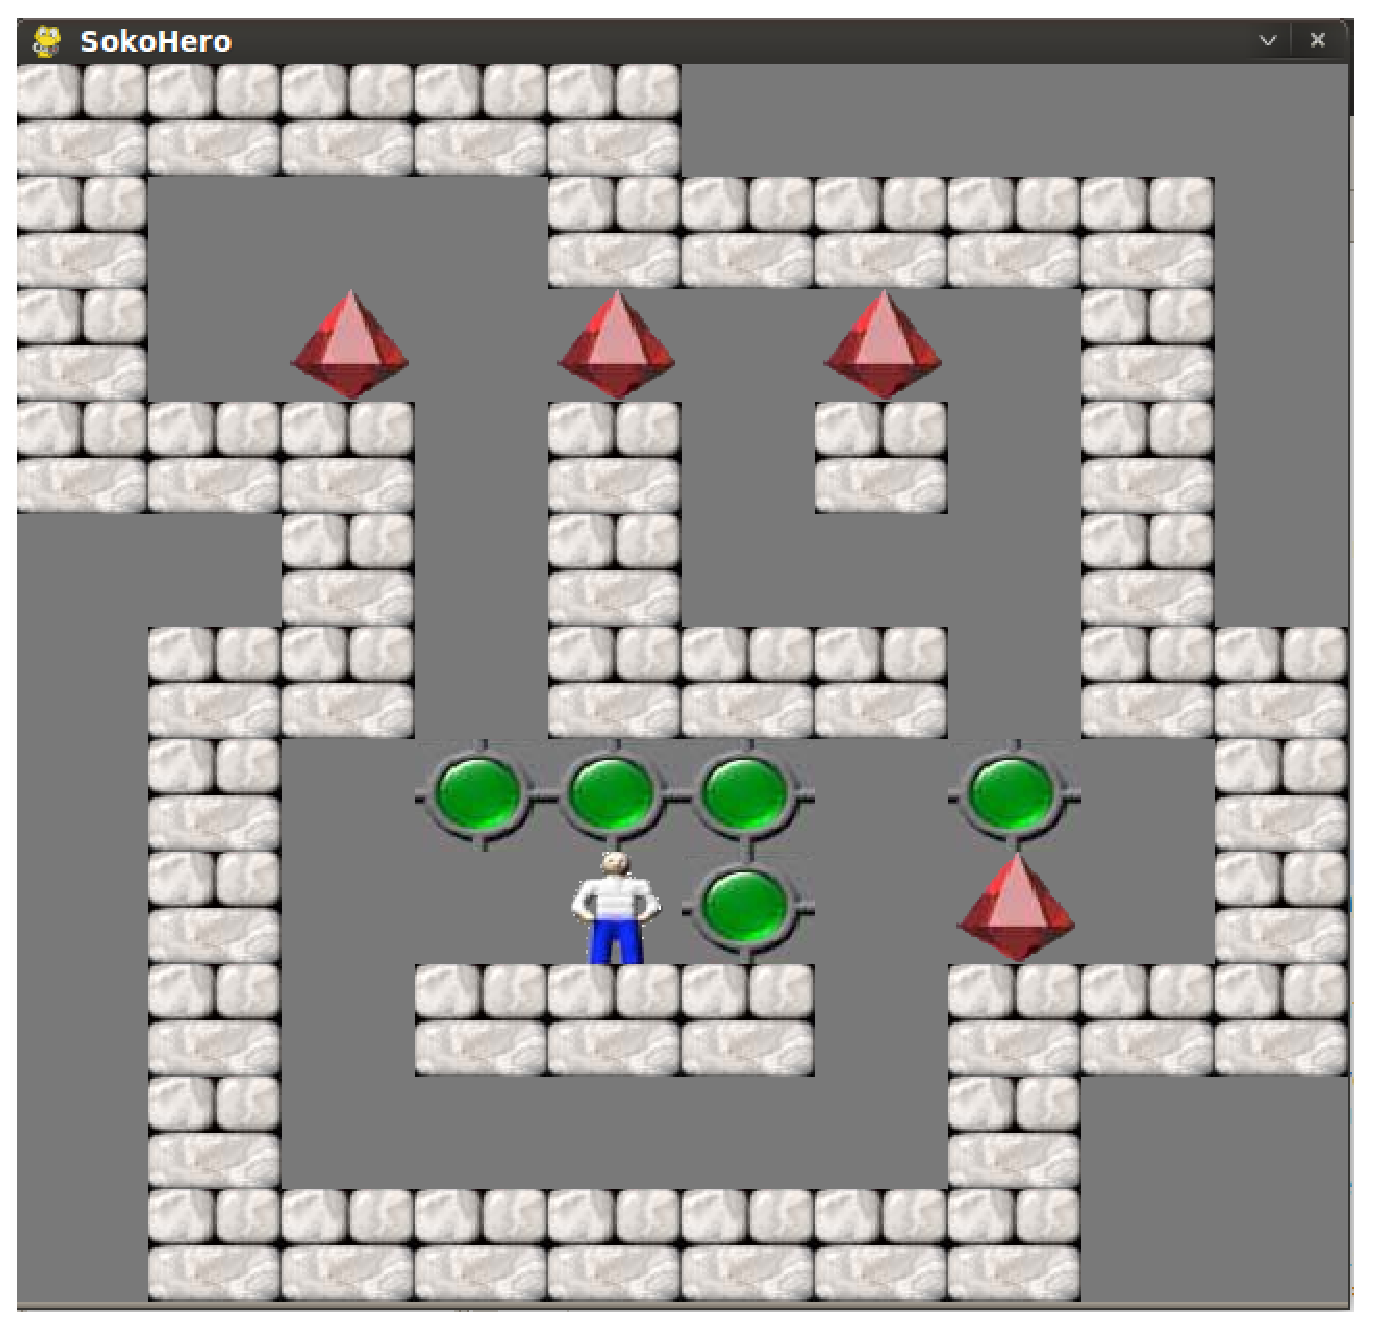
\includegraphics[scale=0.25]{images/sokohero.eps}
\caption{A screenshot of a sokoban game}
\label{fig:sokohero}
\end{figure}


As stated previously the purpose of the game is for the player to push 'Jewel' squares onto 'Goal' squares. That the player is only able to push jewels signifies that if a jewel is at position (x, y), and the player is at position (x - 1, y) then the player will be able to move the jewel to position (x + 1, y) if (x + 1, y) is occupied by an 'Empty' or a 'Goal' square. The same logic applies for other directions.
 
\subsubsection{Challenges faced when solving Sokoban algorithmically}
Given the fact that the player can on average move up, down, left and right, we see that the problem presents a so called branching factor of 4. If an algorithm is able to solve the puzzle in 100 moves, the complexity becomes 4$^{100}$ . 
This enormous complexity, illustrates the need for some sort of heuristics, if the problem is to be solved in an acceptable time frame.
Deadlocks are one of the main challenges faced when trying to solve the Sokoban puzzle. A daedlock is best described as a situation where a jewel is pushed into a position that eliminates the possibility of solving the puzzle, for instance pushing a jewel into a corner. Most current known algorithms that attempt to solve Sokoban due a large amount of processing to try and avoid deadlocks, by using for instance table lookups. One way of solving sokoban however, \cite{franktakes} that can almost avoid any need for deadlock detection, is the so called 'ReversedSolving-algorithm'

\subsubsection{The Reversed-Solving algorithm}
The reversed solving algorithm is based on the idea that all jewel are placed on the goal, and then pulled by the 'Man'/player into the original positions. When the solution has been found, the same path can then be used to push the jewels on to the goals.

The fact that the 'Man' now pulls jewels instead of pushing them, makes it almost impossible to place jewels in deadlock positions (you can for instance not pull a jewel into a corner, or pull next to another jewel in a way that would make it impossible to pull it further).

The algorithm contains the following steps \cite{franktakes}:

\begin{enumerate}
\item Load puzzle, and make a copy to keep track of original position of jewels
\item Place all jewels on the goals
\item As long as the jewels are not placed at the original positions, and the 'Man' is not able to reach his original position, do:
\subitem While condition X is not satisfied:
\subsubitem Pull a jewel to a position where it has not been before
\subitem Change to another jewel, either in random or lexicographical order
\end{enumerate}

\paragraph{The X condition}
The X condition in the above algorithm describes that condition required for the algorithm to switch from one jewel to the next. The following 3 conditions can be used, which all affect the efficiency of the algorithm depending on the puzzle being solved:

\begin{itemize}
\item X1: Afer N steps. N is an integer.
\item X2: When a jewel is at its final position
\item X3: When a jewel is N steps away from a final position
\end{itemize}

